\documentclass[10pt,twocolumn,letterpaper]{article}

\usepackage{cvpr}
\usepackage{times}
\usepackage{epsfig}
\usepackage{graphicx}
\usepackage{amsmath}
\usepackage{amssymb}
\usepackage{algorithm}
\usepackage[noend]{algpseudocode}

\usepackage[breaklinks=true,bookmarks=false]{hyperref}

\cvprfinalcopy

\def\cvprPaperID{****} % *** Enter the CVPR Paper ID here
\def\httilde{\mbox{\tt\raisebox{-.5ex}{\symbol{126}}}}

% Pages are numbered in submission mode, and unnumbered in camera-ready
%\ifcvprfinal\pagestyle{empty}\fi
\setcounter{page}{1}
\begin{document}

%%%%%%%%% TITLE
\title{Image Colorization via Ensemble of Convolutional Neural Networks}

\author{
    Brandon Perez \\
    Carnegie Mellon University \\
    \textit{\small bmperez@andrew.cmu.edu} \\
    \and
    Rohit Banerjee \\
    Carnegie Mellon University \\
    \textit{\small rohitban@andrew.cmu.edu} \\
    \and
    Sohil Shah \\
    Carnegie Mellon University \\
    \textit{\small sohils@andrew.cmu.edu} \\
}

\maketitle

%-------------------------------------------------------------------------------------------
% Abstract
%-------------------------------------------------------------------------------------------

\begin{abstract}
    In this paper, we present a novel technique to automatically colorize grayscale images images using an ensemble of convolution neural networks. The problem of image colorization is to find a hallucination of a grayscale image that produces a reasonable or plausible color version of the image. This is a well-known problem that has been addressed by many other papers, and the solutions can be broken down into two categories: automatic and non-automatic methods. Non-automatic methods require the user to label the image for training, while automatic do not. However, automatic methods all suffer from a common issue: a desaturation bias. That is, the images produced by automatic methods tend to look very desaturated; the colors are dull and not vibrant, which often takes away from the quality. In this paper, we a solution to this problem by training several convolution neural networks for colorization, and using AdaBoost to reduce the desaturation bias of the ensemble of CNNs. This allows for the convenience of automatic methods to be kept, and still produce images with good saturation.
\end{abstract}

%%%%%%%%% BODY TEXT
\section{Introduction}
Image colorization seeks to generate a full color image from an input grayscale scene. The approaches to this problem can be divided into two broad categories: automatic and non-automatic methods. Non-automatic methods require user input and tend to be less computationally expensive compared to automatic methods which operate in the absence of user interaction.

\subsection{Non-Automatic Methods}
Scribble image colorization and Matrix completion rank among the most well studies non-automatic methods \cite{Charpiat2010,Levin2004,Charpiat2008}. Scribble colorization requires the user to annotate the grayscale image with colored lines (“scribbles”). These colors are then propagated in space based on the principle that areas of the image with similar intensities have similar colors \cite{Levin2004}. On a similar vein, matrix completion requires both the grayscale image and a list of pixels with color labels.

\subsection{Automatic Methods}
A shortcoming of non-automatic methods is that different user input is required for each distinct image. Automatic colorization methods overcome this limitation by first training a CNN on an image dataset and then using the trained network to map luminosity values to color values in the image. However, automatic methods tend to be biased towards desaturated background colors \cite{Charpiat2008}.

\subsection{Bias-Variance Reduction of Error by Boosting}
Image colorization is a regression problem, where a generated output, $\hat{Y}$, differs from the true colored image, $Y$, by some error $\xi$. Then, we write the expected value of the squared error as:\newline

$E[\xi^2] = E[(Y-\hat{Y})^2]$ \newline

If we assume the true image, $Y$, can be approximated with some estimation with variance $\sigma^2$, then the expected value of the error can be deconstructed as follows\cite{BiasVar}: \newline

$E[\xi^2] = \sigma^2 + Var[\hat{Y}] + Bias[\hat{Y}]^2$ \newline

Therefore, we can reduce the error by either reducing the variance or the bias \cite{BiasVar}. Boosting is an algorithm to decrease the error of the estimator by reducing bias. Let $\mathcal{H}$ be a set of weak hypotheses estimating $Y$. Then, boosting trains a combination of these $|\mathcal{H}|$ hypotheses to form a new predictor, $\hat{H}$. By training a combination of weaker learners, we can form a new learner with provably lower bias and either identical or lower variance. The difficulty is forming some set of hypotheses that learn unique properties over the data but maintain individually low variance.

\subsection{Ensemble Colorization}
We propose a novel method for image colorization by learning an ensemble of identical CNNs with using Adaptive Boosting to effectively reduce bias of the reconstruction while keeping the method automatic. The algorithm is outlined in figure 1. We will use augmented data to increase the diversity of the estimators generated by the training. We hope to have each CNN performing better on a different subset of tasks, such as one for landscapes and one for people. This will allow us to overcome issues faced in previous research.

\section{Related Work}
\begin{figure}
  \centering
    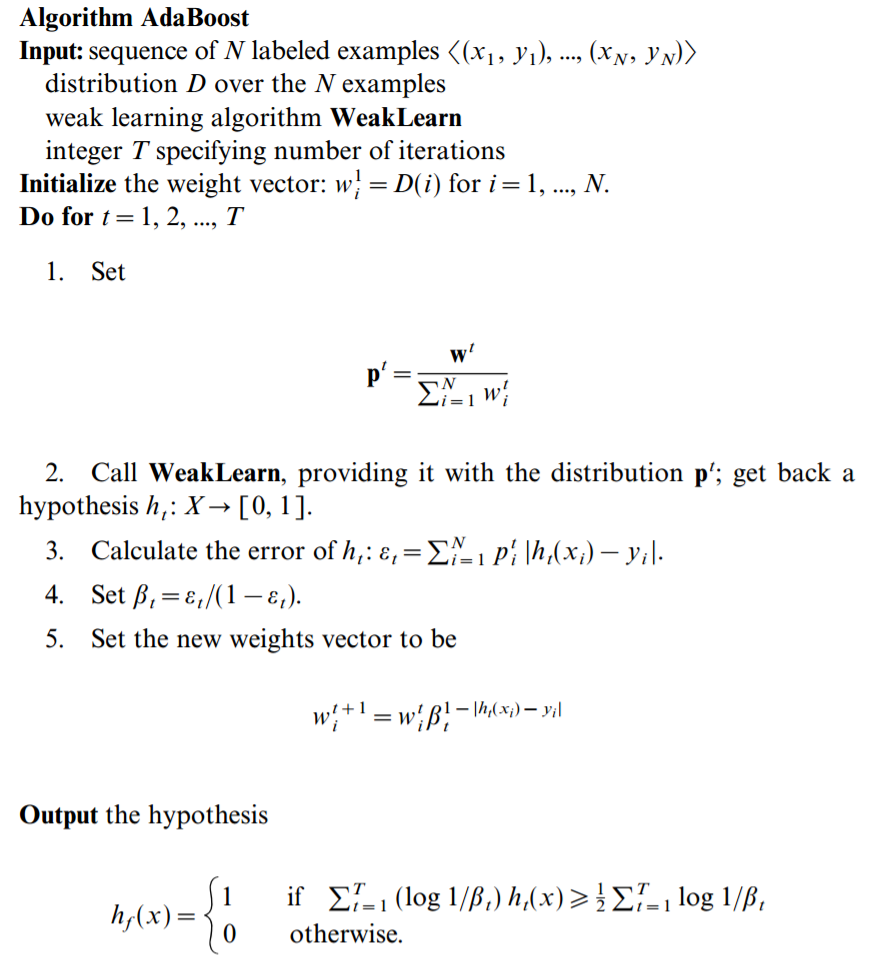
\includegraphics[width=0.5\textwidth]{images/AdaBoost}
  \caption{AdaBoost algorithm \cite{freund1995}}
\end{figure}

A literature study showed us that all automatic colorization techniques
have utilize a Convolutional Neural Networks to learn the prediction functions that map from grayscale to color space. However, they differ in the manner in which they model their color space as well as their CNN architecture.

\subsection{Hypercolumns}
Larsson et al.\cite{Larsson2016} recognize that simply using the final layer of the CNN output to represent features causes the system to be unable to precisely localize features in the image. However, intermediate outputs do not have the correct semantics. Thus they feed a hypercolumn\cite{Hariharan2015} - a vector of activations of all CNN units above the given pixel - into the fully connected layer in order to obtain precise localization data while preserving representational semantics.

\subsection{Class Rebalancing}
In an effort to reduce the bias that Automatice colorization methods have towards desaturated background colors such as beiges and light blues, Zhang et al.\cite{Zhang2016} work off of the inherent multimodal nature of the colorization problem and generate a distribution of colors at each pixel. They then re-weight the loss of each pixel at train time based on pixel color rarity so as to emphasize

\subsection{Colornet}
Colornet is an open source CNN designed to colorize grayscale images implemented using the TensorFlow library\cite{ColorNet}. This network represents the objects in YUV color space and thus maps the luminance Y in grayscale images to the U and V channels \cite{YUVColorSpace}. This model does not create a new CNN to train for the colorization but uses the VGG 16\cite{VGG16}
network along with hypercolumn technology. It must be noted that this model produces desaturated output images. However, we will be using this model as a component in out ensemble system due to its ease of use.
d
\section{Approach and Algorithm}

\begin{figure*}
  \centering
    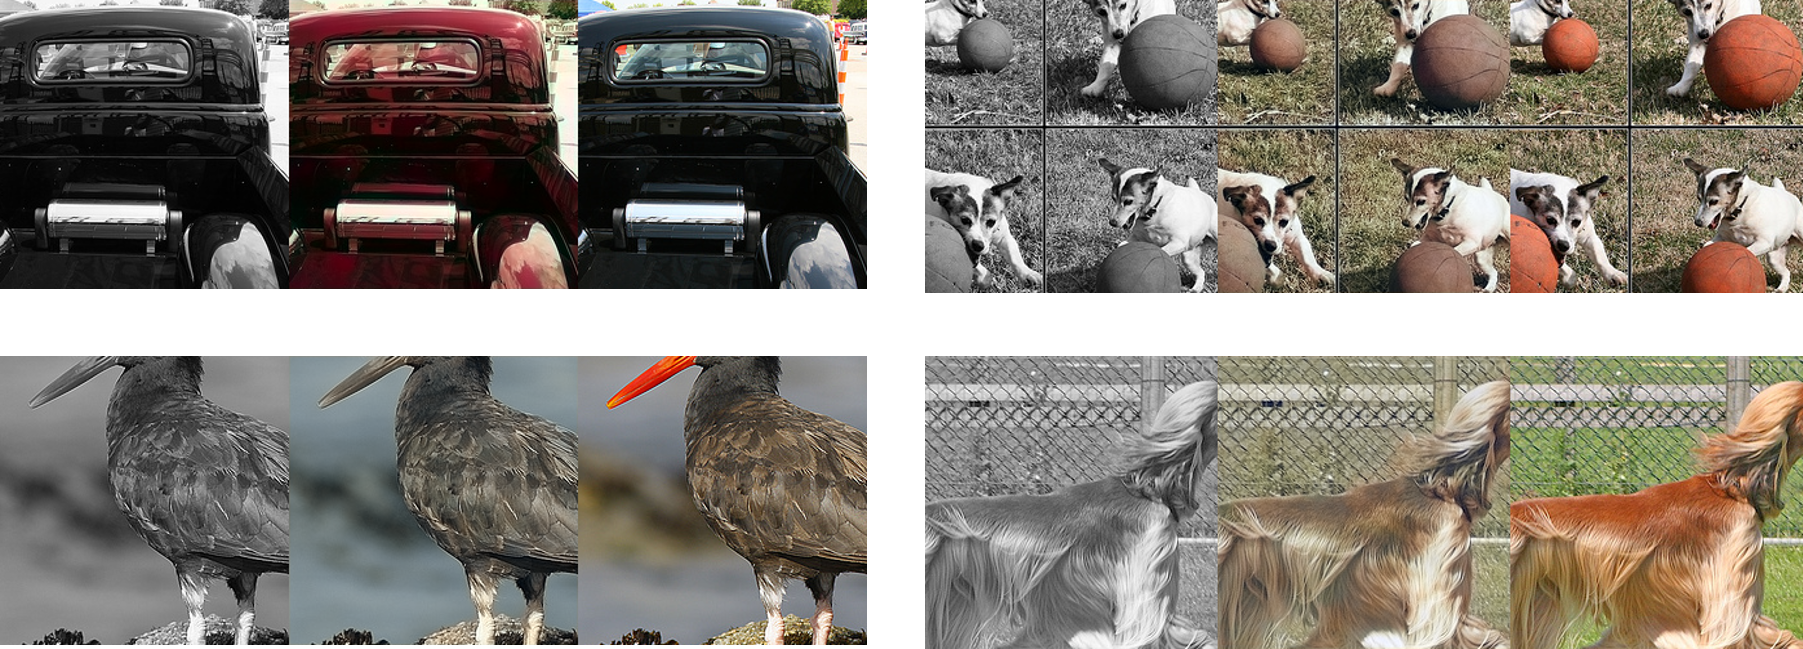
\includegraphics[width=1\textwidth]{images/colornet}
  \caption{Colornet colorization results \cite{ColorNet}. Left is the grayscale input, center is the reconstructed image, and right is ground truth. Each image shows high bias. The image on the top left shows a large bias towards red, and the other three images have high desaturation.}
\end{figure*}

We will be using instances of the Colornet\cite{ColorNet} model in  our ensemble system. Using a single Colornet model will produce desaturated output images thus we plan to augment our dataset by performing Gaussian and contrast transforms on our input dataset. Each instance of the Colornet will then be trained on a subset of the augmented dataset in an effort to make it learn a separate section of the prediction function that maps from the grayscale to YUV colorspace. Thus in our ensemble model, we treat each instance as a weak learners whose outputs we weight via Adaptive Boosting in order to produce a single output image.

\subsection{Dataset}
The network is tested and trained on a subset of the ImageNet database \cite{Russakovsky2015}. The images are rescaled to 256x256 for consistency and first converted to grayscale. We perform data augmentation by creating duplicates of the images at higher and lower contrast, different amounts of blur, and other label preserving transformations. This increases diversity of the hypotheses learned by the ensemble. A potential bottleneck may be how many images we can train on, as the previous work uses powerful GPU based clusters to train on millions of images \cite{Hariharan2015, DeepColorization}. The test images will be taken from the same synsets of the ImageNet database as was trained on to keep consistency and prevent us from needing to train on too large a number of images.

\subsection{Label Invariant Data Augmentation}
Data augmentation commonly used in convolutional neural networks to add generality to the estimator, reduce overfitting, and increase the size of the dataset. In our case, we wish to train an ensemble of convolutional neural nets, where each CNN is trained by a different set of transformations. This will allow us to recombine the results via boosting for lower error.

\subsection{Network structure}
We use an ensemble of n identical convolutional neural networks, following similar design to that seen in \cite{Hariharan2015, DeepColorization}. In this case, $n$ will be determined experimentally in order to get a good trade-off between bias and variance. The augmented data is placed in a sample pool of size $m$. We then bootstrap $n$ sets of $m$ training examples randomly with replacement from the sample pool. This method diversifies the concepts learned by each of the CNNs, allowing them each to converge to different solutions. Then, the AdaBoost method is used to train the ensemble and re-weight the CNN coefficients. The final reconstruction will consist of a linear combination of the n CNNs.

We will evaluate the prediction by calculating the mean square error of the reconstructed output and the original image. Training finishes when MSE is less than a threshold $\epsilon$. The bias of the individual CNNs is expected to be high. With a diverse enough set of generated hypotheses, boosting provably reduces both bias and variance.

\section{Experiments and Progress}

For the midpoint of the project, we focused on the individual, weaker classifier. This CNN, called Colornet, is based off of VGG-16, a popular network for the tasks of segmentation and hallucination. It functions via convolutions and pooling, then deconvolution and unpooling layers. This allows it to reconstruct a hallucinated image, so it is perfect for this task. At the time, we have found many pre-trained models for VGG-16 for the task of colorization, so we will not have to train the model from scratch, as this usually will take prohibitively long. Furthermore, boosting does not require that the ensemble of learners be trained during the boosting; instead, we can train our set of hypotheses first, then tune the hyperparameters of the boosting algorithm to also save time.

\subsection{Hardware and Software Stack}
The ensemble colorization system is very computationally expensive. VGG-16 is a large network with too many parameters to be trained in reasonable time from scratch on regular CPUs. To solve this, we will train starting from pre-trained base models and train on a GPU. For this project, we use a desktop with a NVIDIA 980Ti GPU to perform fast training. The training is accelerated by cuDNN with TensorFlow. Using TensorFlow greatly minimizes our implementation and debugging time. Furthermore, the Colornet model is based off of TensorFlow. Therefore, we can easily add to and modify the existing code.

Since we use TensorFlow, we also write our entire preprocessing and data augmentation pipeline in Python. This makes it very easy to quickly prototype and modify hyperparameter settings for the system. Also, it allows us to use many existing Python libraries for data augmentation and image processing. We also write the boosting part of the code in Python and Tensorflow in order to quickly prototype it.

\subsection{Running Colornet}
We spent the first half of the project working on integrating Colornet into our project. We use its pretrained model and train on top of it using our own training samples. Results for the pretrained model can be seen in figure 2. We have also successfully designed the boosting algorithm for use with the CNNs, and have a plan for implementing it together. We have not made as much progress as we wanted here because of issues in running Colornet in the beginning. It required some modification and preprocessing before we got it fully functional, so these issues slowed us down.

\subsection{Data Augmentation}
We have come up with several different data augmentation techniques. The simplest technique is to simply vary the contrast in the grayscale images. We hope that by doing this, we learn different cases in which images need more contrast or less contrast. We could also vary the saturation of the label images in order to increase the saturation of some predictors. By doing this on an ensemble, we would be able to for some learners to have high saturation and others lower saturation. Then the weighted recombination will allow us to get a result that is closer to the ground truth.

Another augmentation technique is applying Gaussian filters to the grayscale image to blur them. By doing this, we wish to function better on inputs with less hue variation and high value variation. The blurring will allow us to reduce the high frequency content in the input images in order to better predict images with large regions of continuous color.

\section{Conclusion}
Thus far we have been able to successfully train and test instance of the Colornet system. We are also into the process of training our implementation of our boosting algorithm that will combine the outputs of the individual Colornet instances. We expect that if we are able to successfully partition the prediction function among the weak learners it is likely that we will be able to reduce the bias towards desaturated colors in out output images.

We believe that the key difficulty at this stage in the process lies in successfully calculating the weights for each of the weak learners in out ensemble system. As there was a lack of literature regarding the usage of ensembles for image colorization we lack information to formulate a concrete hypothesis regarding which of the augmented datasets are likely to produce a trained CNN with greater weight.

Moreover, if we are successful in this endeavour, we will have proved that we can use an ensemble of very basic colorization networks to eliminate colorization bias. This would open up further avenues for future research as the ensemble could be combined with other bias reducing algorithms such as class rebalancing\cite{Zhang2016} in an effort to further improve the fidelity of the recolored grayscale images.

{\small
\bibliographystyle{ieee}
\bibliography{egbib}
}

\end{document}
